% IEEE Conference Paper — Remaining Useful Life Prediction
% Phase 1 (ML) + Phase 2 (DL) Combined Report
\documentclass[conference]{IEEEtran}

\usepackage{amsmath,amssymb}
\usepackage{graphicx}
\usepackage{booktabs}
\usepackage{hyperref}
\usepackage{cite}
\usepackage{multirow}

\graphicspath{{../results/phase2/figures/}}

\title{Remaining Useful Life Prediction of Aircraft Engines\\Using Machine Learning and Deep Learning on C-MAPSS FD001}

\author{
  \IEEEauthorblockN{Yogesh Modi, Abhishek Kumar Patel, Kapish Rohilla, Vikash Kumar, Prateek Shakya}
  \IEEEauthorblockA{Department of Computer Science\\University Course Project — Applied Machine Learning / Deep Learning}
}

\begin{document}
\maketitle

\begin{abstract}
Predicting the Remaining Useful Life (RUL) of aircraft engines enables
condition-based maintenance and reduces unplanned downtime.  This work
addresses the problem on the NASA C-MAPSS FD001 benchmark, which provides
multivariate sensor time series from 100 training and 100 test turbofan
engines run to failure.  In Phase~1 we established baselines with
engineered rolling-window features and four regression models (OLS,
Elastic Net, Random Forest, Gradient Boosting), achieving a best
validation MAE of 25.03 cycles (Random Forest).  Phase~2 replaces the
hand-crafted pipeline with end-to-end deep learning: LSTM, GRU, 1D-CNN
and Transformer architectures trained on 30-cycle sliding windows, plus a
hybrid stacking model that combines deep-learning embeddings with
traditional features.  Systematic ablation studies over window length,
input features, RUL target capping, model capacity, regularisation and
architecture quantify each design choice.  The best single deep-learning
model (LSTM) reduces the validation MAE to 19.41 cycles, a 22\%
improvement over the Phase~1 baseline, while the stacking hybrid achieves
21.48 cycles with more stable predictions across RUL bands.  All results
are reproducible with seed~42 and all code is publicly available.
\end{abstract}

\section{Introduction}
\label{sec:introduction}

Remaining Useful Life (RUL) prediction estimates how many more operating
cycles a machine can sustain before failure.  Accurate RUL estimates
enable condition-based maintenance, reducing both unplanned failures and
unnecessary preventive replacements~\cite{saxena_2008_damage_prognosis}.

We study the NASA Commercial Modular Aero-Propulsion System Simulation
(C-MAPSS) FD001 dataset, a widely used benchmark comprising 100 training
and 100 test turbofan engines.  Each engine is monitored by 21 sensors
and 3 operational settings over its full run-to-failure trajectory.
After removing 7 constant or near-constant sensors, 14 informative
channels remain.

\subsection{Phase 1 Recap}
In Phase~1 we constructed hand-crafted rolling-window features (mean,
standard deviation and slope over the most recent 10 cycles) for each
sensor channel, yielding 57 features per observation.  Four regression
models were trained on 80 engines and evaluated on 100 fixed validation
points from 20 held-out engines:

\begin{table}[h]
\centering
\caption{Phase 1 validation results (100 fixed points)}
\label{tab:phase1_results}
\begin{tabular}{lcc}
\toprule
Model & MAE & RMSE \\
\midrule
OLS & 32.86 & 42.92 \\
Elastic Net & 31.66 & 41.77 \\
Random Forest & 25.03 & 40.17 \\
Gradient Boosting & 26.12 & 40.17 \\
\bottomrule
\end{tabular}
\end{table}

Key weaknesses identified in Phase~1: (a) systematic under-prediction
for engines with true RUL above 200 cycles (mean error approximately
$-120$ cycles for linear models), (b) the 10-cycle rolling window
captures only very recent sensor behaviour, and (c) RMSE substantially
exceeds MAE, indicating a few large errors dominate.

\subsection{Phase 2 Contributions}
Phase~2 addresses these weaknesses with four contributions:
\begin{enumerate}
  \item \textbf{Sequence models.} LSTM and GRU networks learn temporal
    patterns directly from 30-cycle sliding windows, removing the need
    for hand-crafted features.
  \item \textbf{Alternative architectures.} A 1D-CNN and a Transformer
    encoder provide complementary inductive biases (local convolution
    versus global self-attention).
  \item \textbf{Hybrid stacking.} A second-stage Random Forest combines
    deep-learning predictions with traditional rolling features in an
    out-of-fold stacking framework.
  \item \textbf{Ablation studies.} Seven controlled experiments quantify
    the impact of window length, input features, RUL capping, model
    capacity, regularisation, architecture choice and hybrid components.
\end{enumerate}

The rest of this paper is organised as follows.
Section~\ref{sec:literature} reviews related work.
Section~\ref{sec:dataset} describes the dataset and preprocessing.
Sections~\ref{sec:recurrent}--\ref{sec:hybrid} present the four model
families.  Section~\ref{sec:ablations} reports the ablation studies.
Section~\ref{sec:results} gives the final evaluation on both validation
and held-out test sets with bootstrap confidence intervals.
Section~\ref{sec:conclusion} concludes.

\section{Deep Learning Literature}
\label{sec:literature}

The C-MAPSS benchmark was introduced as a run-to-failure simulation of
turbofan degradation \cite{saxena_2008_damage_prognosis}.  Its engine-indexed
multivariate trajectories make it a natural test bed for models that learn
temporal context rather than treating observations as independent rows.
Long short-term memory (LSTM) networks use gated memory to preserve useful
information over long intervals \cite{hochreiter_1997_lstm}; gated recurrent
units (GRUs) provide a smaller alternative \cite{cho_2014_gru}.  In contrast,
temporal convolutional networks (TCNs) use causal convolutions and a finite
receptive field \cite{bai_2018_tcn}, while the Transformer replaces recurrence
with attention \cite{vaswani_2017_transformer}.

RUL studies commonly use convolutional encoders because local changes in
sensor trajectories are predictive.  Babu et al. proposed a deep CNN
regression approach for C-MAPSS \cite{babu_2016_dcnn}, and Li et al. studied
deep convolutional features for prognostics \cite{li_2018_dcnn}.  LSTM-based
RUL work further demonstrated that a sequence representation can model
degradation history \cite{zheng_2017_lstm}.  Attention and CNN--recurrent
hybrids are attractive extensions, but their extra parameters are a material
risk when only 100 engines are available.  The literature also frequently
uses a piecewise-linear cap near 125 cycles: this reduces the influence of
uncertain early-life labels, but can remove information needed to correct the
high-RUL underprediction seen in our uncapped Phase 1 baseline.

\begin{table}[t]
\caption{Scope of the reviewed literature. ``n/a'' means that the source or
the accessible report did not state the item unambiguously.}
\label{tab:literature}
\centering
\scriptsize
\resizebox{\columnwidth}{!}{%
\begin{tabular}{p{0.25\columnwidth}p{0.18\columnwidth}p{0.15\columnwidth}p{0.28\columnwidth}}
\hline
Source & Model & Subset & Limitation \\
\hline
Babu et al. & CNN & FD001--FD004 & Representation-sensitive \\
Li et al. & CNN & FD001--FD004 & Preprocessing-sensitive \\
Zheng et al. & LSTM & FD001--FD004 & Capping discards high-RUL detail \\
Bai et al. & TCN & n/a & Receptive-field dependent \\
Vaswani et al. & Transformer & n/a & Attention cost grows with length \\
\hline
\end{tabular}}
\end{table}

Unlike Phase 1's ten-cycle rolling summaries, a window model receives the
ordered sensor values and can learn interactions between trends, transients,
and delayed effects.  Reported windows vary by task, and there is no
universally optimal length: short windows miss slow degradation while long
windows increase padding, computation, and overfitting.  These observations
motivate a controlled comparison of recurrent, convolutional, attention, and
hybrid representations on the same engine split.

\section{Dataset and Sequence Preprocessing}
\label{sec:preprocessing}

We used the NASA C-MAPSS FD001 data.  Each observation contains an engine
identifier, cycle, three operating settings, and 21 sensor measurements.
Seven constant or near-constant columns were removed, leaving the 14 sensors
used by the sequence models.  The training RUL target was
\[
y_{i,t}=\max_{u \in i}(u)-t,
\]
where $i$ denotes an engine and $t$ its current cycle.  The 100 validation
cutoffs were kept fixed and the split was performed by engine: 80 engines
were used for fitting and 20 for validation.  Consequently, no window
contained observations from both partitions.

The scaler was fitted only on observations from the 80 training engines.
For sensor $j$, the transformed value was
$z_{i,t,j}=(x_{i,t,j}-\mu_j)/\sigma_j$.  At cycle $t$, a window of length $w$
was constructed as
\[
X_{i,t}=[z_{i,t-w+1},\ldots,z_{i,t}],
\]
using only observations at or before $t$.  If fewer than $w$ observations
were available, the first observed vector was repeated on the left.  Thus
short test engines remain usable without look-ahead or deletion.  A cap can
be applied to training targets as $\tilde y=\min(y,c)$, but the default
pipeline leaves targets uncapped and every evaluation uses the true RUL.

Models were evaluated in the exact order of the 100 fixed validation points.
We reported mean absolute error (MAE) and root mean squared error (RMSE) in
cycles, together with early-life ($y>125$) and late-life ($y\leq125$)
breakdowns.  Test windows were generated only at each engine's final
observed cycle; their labels were not used during model development.

\section{Recurrent Models and Training Protocol}
\label{sec:recurrent}

\subsection{Recurrent networks and their gradients}
A recurrent network reads a window $x_1,\dots,x_T$ ($T=30$, $x_t\in\mathbb{R}^{14}$) and updates a hidden state
\begin{equation}
h_t=\tanh\!\left(W_x x_t+W_h h_{t-1}+b\right),
\end{equation}
where $W_x$ and $W_h$ are the input and recurrent weight matrices and $b$ is a bias.  The prediction is $\hat y=w^\top h_T+b_o$, with head weights $w$ and bias $b_o$.  Training by backpropagation through time (BPTT) unrolls the recurrence, and the gradient of the loss $\mathcal{L}$ with respect to an early state is
\begin{equation}
\frac{\partial \mathcal{L}}{\partial h_k}=\frac{\partial \mathcal{L}}{\partial h_T}\prod_{t=k+1}^{T}\frac{\partial h_t}{\partial h_{t-1}} .
\end{equation}
If the norm of each Jacobian factor is below one, the product shrinks geometrically with $T-k$ (vanishing gradients) and distant cycles stop influencing learning; if it is above one, the product grows (exploding gradients)~\cite{pascanu_2013_difficulty}.

\textbf{LSTM.}  The long short-term memory (LSTM) cell adds a cell state $c_t$ that is updated additively~\cite{hochreiter_1997_lstm,gers_2000_forget}:
\begin{align}
i_t&=\sigma(W_i[x_t,h_{t-1}]+b_i), & f_t&=\sigma(W_f[x_t,h_{t-1}]+b_f),\\
o_t&=\sigma(W_o[x_t,h_{t-1}]+b_o'), & g_t&=\tanh(W_g[x_t,h_{t-1}]+b_g),\\
c_t&=f_t\odot c_{t-1}+i_t\odot g_t, & h_t&=o_t\odot\tanh(c_t),
\end{align}
where $i_t$, $f_t$, $o_t$ are the input, forget and output gates, $g_t$ is the candidate update, $\sigma$ is the logistic function and $\odot$ is element-wise multiplication.  Because $\partial c_t/\partial c_{t-1}=f_t$ (a gate in $(0,1)$ rather than a repeated weight matrix), the gradient along the cell path is not forced to vanish.

\textbf{GRU.}  The gated recurrent unit (GRU) merges cell and hidden state and uses two gates~\cite{cho_2014_gru}:
\begin{align}
z_t&=\sigma(W_z[x_t,h_{t-1}]+b_z), & r_t&=\sigma(W_r[x_t,h_{t-1}]+b_r),\\
\tilde h_t&=\tanh(W_h[x_t,r_t\odot h_{t-1}]+b_h), & h_t&=(1-z_t)\odot h_{t-1}+z_t\odot\tilde h_t,
\end{align}
with update gate $z_t$ and reset gate $r_t$.  A GRU has three weight blocks per layer instead of four, hence fewer parameters.

\subsection{Training protocol}
The loss was the mean squared error on the scaled target,
$\mathcal{L}=\frac{1}{N}\sum_{n=1}^{N}\big(\hat y_n-y_n/100\big)^2$, with the true uncapped RUL $y_n$.  We used AdamW~\cite{loshchilov_2019_adamw}, whose update is
\begin{equation}
\theta\leftarrow\theta-\eta\left(\frac{\hat m}{\sqrt{\hat v}+\epsilon}+\lambda\theta\right),
\end{equation}
where $\theta$ are the weights, $\eta=10^{-3}$ the learning rate, $\hat m,\hat v$ the bias-corrected first and second moment estimates of the gradient, and $\lambda$ the weight decay.  The decay term is applied to the weights directly and is not passed through the adaptive scaling, which is what \emph{decoupled} means; with plain L2 regularization the penalty would be rescaled by $1/\sqrt{\hat v}$.  Dropout~\cite{srivastava_2014_dropout} multiplies the hidden vector by a Bernoulli mask, $\tilde h=m\odot h/(1-p)$ with $m_j\sim\mathrm{Bernoulli}(1-p)$, between recurrent layers and before the output layer.  Gradient clipping replaces a gradient $g$ by $g\cdot\min(1,\tau/\lVert g\rVert_2)$ with $\tau=1$~\cite{pascanu_2013_difficulty}.  Early stopping kept the weights of the epoch with the lowest mean absolute error over all windows of the 20 validation engines, with a maximum of 60 epochs and a patience of 8 epochs.  Because both the stopping epoch and the final configuration were chosen on these engines, the validation scores are slightly optimistic; the held-out test set is the unbiased check.  Training used the 80 training engines (16,390 windows) with batch size 256 and seed 42; windows of one engine overlap by 29 of 30 cycles, so the effective sample size is close to 80 rather than 16,390.

Each factor was varied alone around a baseline of two layers, 64 hidden units, dropout 0.2, weight decay $10^{-4}$ and patience 8, for both cell types.  A final configuration per model was chosen by the lowest validation-engine window MAE (differences below 0.05 cycles went to the smaller model), a rule fixed before the results were inspected; the 100 fixed validation points were not used for selection.

\subsection{Results}
Table~\ref{tab:reg} lists the validation-engine window MAE for every setting and Fig.~\ref{fig:sweeps} plots it together with the training MAE.  The selection rule chose a one-layer LSTM with 64 units and dropout 0.2 (20,545 parameters; \texttt{config\_lstm.json}) and a two-layer GRU with 64 units and dropout 0.3 (40,385 parameters; \texttt{config\_gru.json}).  Both used AdamW with weight decay $10^{-4}$.

Early stopping was the only regularizer with a clear effect.  Training for a fixed 60 epochs and keeping the last epoch raised the window MAE from 26.87 to 31.15 cycles (GRU) and from 28.42 to 31.95 (LSTM) while the training MAE fell to about 7 cycles.  Dropout and weight decay moved the score by at most 0.68 and 0.07 cycles, which is smaller than the seed-to-seed variation of a fixed configuration (26.78, 27.01, 27.20 for the GRU; 26.38, 27.17, 27.22 for the LSTM), so these effects cannot be separated from noise.  Weight decay is nearly inert because AdamW shrinks the weights by only $\eta\lambda=10^{-7}$ per step.  Gradient clipping was not needed to prevent divergence: the mean gradient norm per epoch peaked at 1.57 (GRU) and 1.31 (LSTM) with clipping at 1.0, and at 1.13 and 0.99 without it.

\begin{table}[t]
\centering
\caption{Validation-engine window MAE (cycles) for each one-factor change. Bold marks the baseline value. Single runs, seed 42.}
\label{tab:reg}
\footnotesize
\begin{tabular}{llcc}
\toprule
Factor & Value & GRU & LSTM\\
\midrule
Dropout & 0 & 26.95 & 28.68\\
 & 0.1 & 26.97 & 28.66\\
 & \textbf{0.2} & \textbf{26.87} & \textbf{28.42}\\
 & 0.3 & 26.78 & 28.01\\
 & 0.5 & 27.16 & 28.23\\
\midrule
Weight decay & 0 & 26.86 & 28.40\\
 & $10^{-5}$ & 26.86 & 28.40\\
 & \textbf{$10^{-4}$} & \textbf{26.87} & \textbf{28.42}\\
 & $10^{-3}$ & 26.80 & 28.44\\
\midrule
Patience & 3 & 27.39 & 28.50\\
 & \textbf{8} & \textbf{26.87} & \textbf{28.42}\\
 & 15 & 26.87 & 28.42\\
 & none (60 ep.) & 31.15 & 31.95\\
\midrule
Hidden units & 32 & 27.19 & 27.39\\
 & \textbf{64} & \textbf{26.87} & \textbf{28.42}\\
 & 128 & 27.77 & 27.06\\
\midrule
Layers & 1 & 27.01 & 26.38\\
 & \textbf{2} & \textbf{26.87} & \textbf{28.42}\\
 & 3 & 26.77 & 27.72\\
\bottomrule
\end{tabular}
\end{table}

\begin{figure*}[t]
\centering
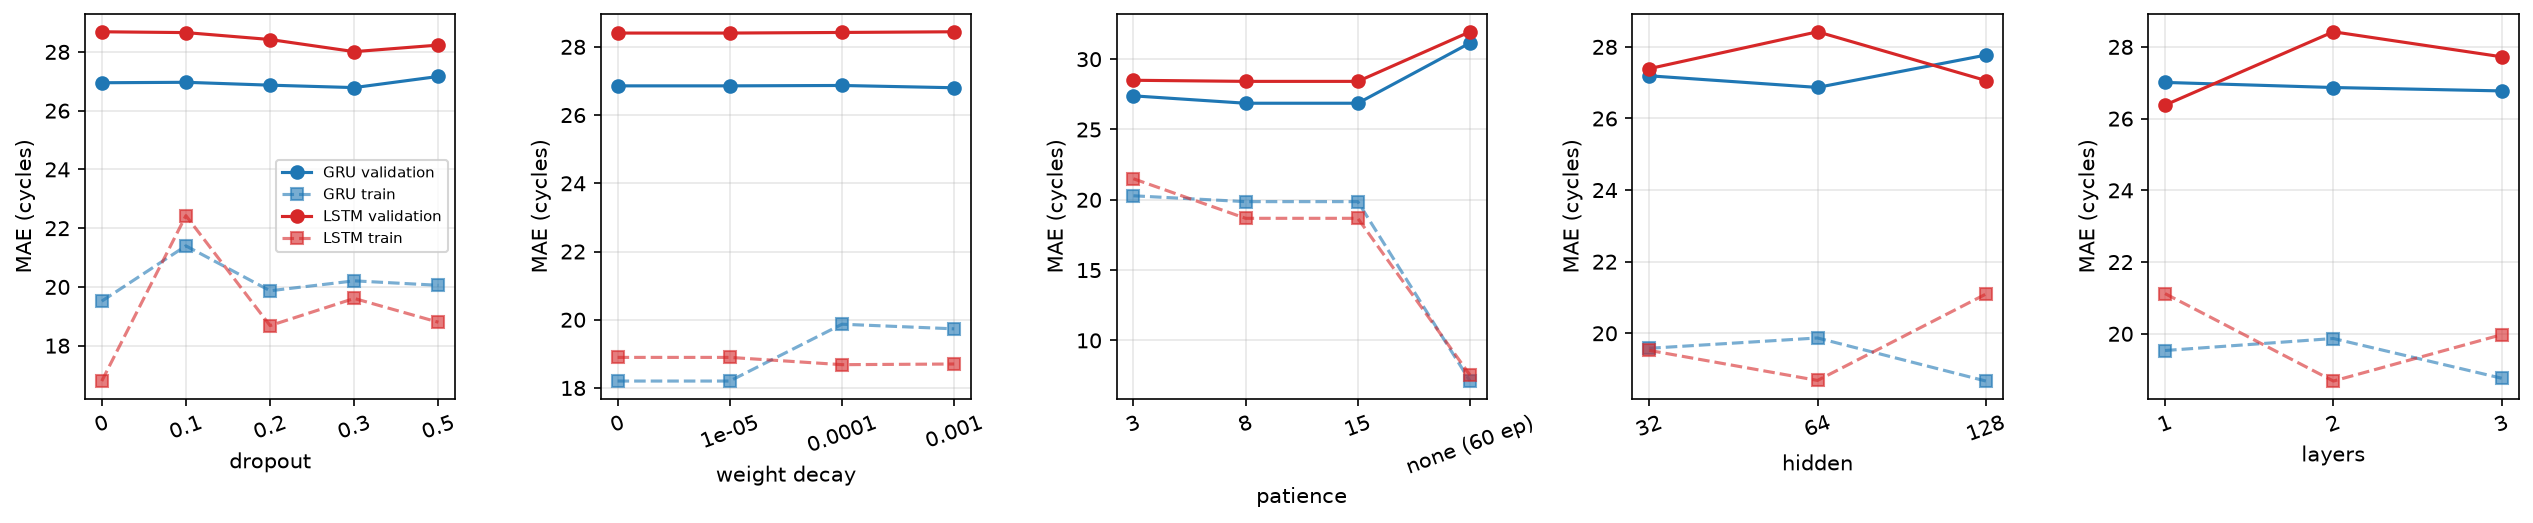
\includegraphics[width=\textwidth]{../results/phase2/figures/rnn_regularization_sweeps.png}
\caption{Validation-engine window MAE (solid) and training MAE in evaluation mode (dashed) against each setting; one run per point.}
\label{fig:sweeps}
\end{figure*}

Table~\ref{tab:final} gives the scores of the chosen models on the 100 fixed validation points.  The three-seed means of the LSTM and the GRU (20.14 and 22.98 MAE) are below the Random Forest value of Phase~1 (25.03), by 4.89 and 2.05 cycles, which is larger than the seed standard deviations; the RMSE falls from 40.17 to 33.18 (LSTM) and 36.61 (GRU).  The early-life MAE (true RUL above 125) remains high at 43.7 and 43.3 cycles for the saved models.  In the band above 200 cycles (five points) the mean error is $-124.7$ (LSTM) and $-115.8$ (GRU) cycles, so the underprediction of Phase~1 is not removed; five points are too few for a firm conclusion.  At the matched two-layer, 64-unit setting the LSTM has 53,825 parameters against 40,385 for the GRU and needs 1.48 s per epoch against 1.14 s on one CPU thread.  The seed 42 baselines of the two cell types differ by one cycle of MAE (21.83 and 22.83), within seed noise, so the evidence for one cell type is weak.

\begin{table}[t]
\centering
\caption{Chosen models on the 100 validation points. Mean $\pm$ standard deviation over seeds 42, 43, 44; early and late MAE are for the saved seed 42 model. The Random Forest row is the Phase~1 result.}
\label{tab:final}
\footnotesize
\begin{tabular}{lcccc}
\toprule
Model & MAE & RMSE & Early MAE & Late MAE\\
\midrule
LSTM (1 layer, 64) & $20.14\pm1.46$ & $33.18\pm2.46$ & 43.73 & 12.55\\
GRU (2 layers, 64) & $22.98\pm0.49$ & $36.61\pm0.90$ & 43.34 & 17.49\\
Random Forest (Phase 1) & 25.03 & 40.17 & 49.33 & 18.17\\
\bottomrule
\end{tabular}
\end{table}

\begin{figure}[t]
\centering
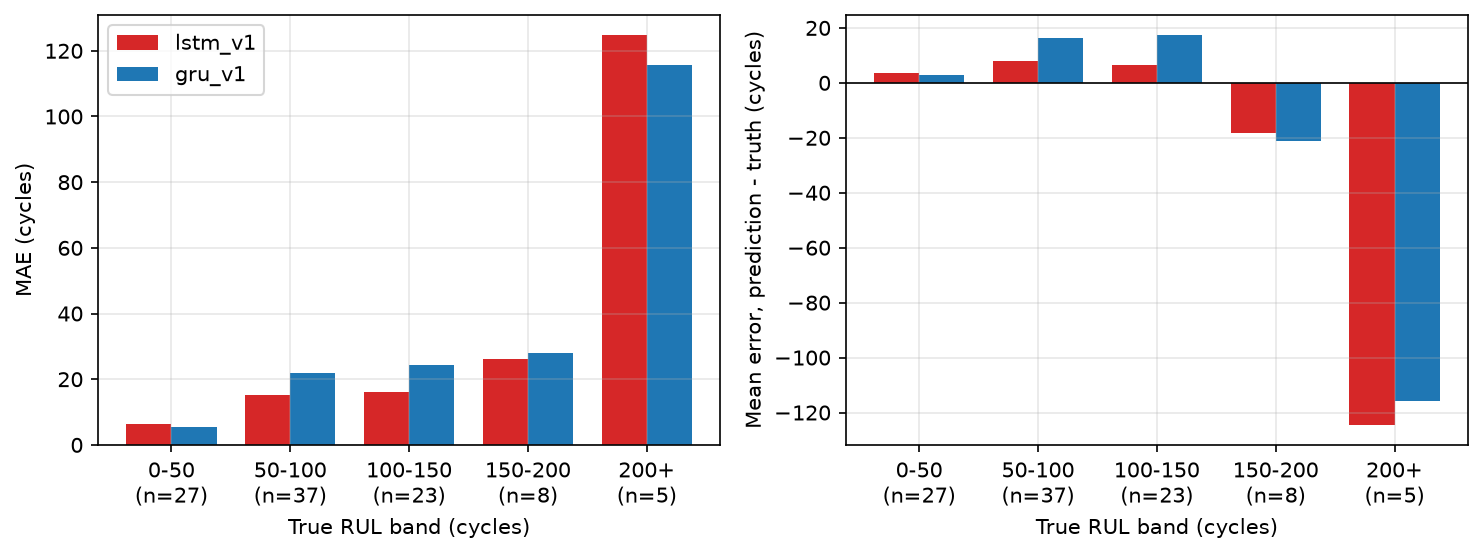
\includegraphics[width=\columnwidth]{../results/phase2/figures/rnn_error_by_band.png}
\caption{Error by true-RUL band for the saved models, with the number of validation points per band.}
\label{fig:bands}
\end{figure}

\section{Convolutional and Transformer Models}
\label{sec:cnn_transformer}

Both models read the same window as the recurrent networks of Section~\ref{sec:recurrent}: $X=(x_1,\dots,x_T)$ with $T=30$ cycles and $x_t\in\mathbb{R}^{14}$, standardised with training-engine statistics.  Each model maps $X$ to a pooled vector $z\in\mathbb{R}^{d}$ and predicts $\hat y=w^\top z+b$, trained with the same loss, optimiser (AdamW~\cite{loshchilov_2019_adamw}), early stopping and selection rule as the recurrent models.

\subsection{One-dimensional CNN}
A convolutional layer with kernel size $k$ and dilation $\delta$ computes, for output channel $c'$ and position $t$,
\begin{equation}
h^{(c')}_t=\mathrm{ReLU}\!\Big(b_{c'}+\sum_{c=1}^{C_{\mathrm{in}}}\sum_{j=-(k-1)/2}^{(k-1)/2} w_{c',c,j}\,x^{(c)}_{t+\delta j}\Big),
\end{equation}
where $w$ are the learned filters, $b$ the biases and $C_{\mathrm{in}}$ the number of input channels, with zero padding at the window ends.  Stacking $L$ layers with dilations $\delta_1,\dots,\delta_L$ gives every position a receptive field of
\begin{equation}
R=1+(k-1)\sum_{l=1}^{L}\delta_l
\end{equation}
cycles.  Global average pooling $z=\frac{1}{T}\sum_{t}h_t$ then summarises the window.  Symmetric padding is safe because a window already ends at the current cycle, so every position lies in the past.  The starter model ($L=2$, $k=5$, $\delta=1$) had $R=9$.  We changed one factor at a time: normalisation (batch~\cite{ioffe_2015_batchnorm} or layer~\cite{ba_2016_layernorm}), residual connections $h\leftarrow h+F(h)$~\cite{he_2016_resnet}, pooling (average, maximum, last step), dilation, depth and kernel size.  Convolutional regression networks have been used for RUL before~\cite{babu_2016_dcnn,li_2018_dcnn}, and dilated convolutions are the basis of temporal convolutional networks~\cite{bai_2018_tcn}.

\subsection{Transformer encoder}
The Transformer replaces recurrence by self-attention~\cite{vaswani_2017_transformer}.  A linear layer projects each $x_t$ to $d_{\mathrm{model}}=32$ and a positional encoding is added, because attention alone ignores order:
\begin{align}
\mathrm{PE}(t,2i)&=\sin\!\big(t/10000^{2i/d_{\mathrm{model}}}\big),\\
\mathrm{PE}(t,2i{+}1)&=\cos\!\big(t/10000^{2i/d_{\mathrm{model}}}\big).
\end{align}
With $Q$, $K$, $V$ the query, key and value projections of the sequence and $d_k$ the key size, one head computes
\begin{equation}
\mathrm{Attention}(Q,K,V)=\mathrm{softmax}\!\Big(\frac{QK^\top}{\sqrt{d_k}}\Big)V,
\end{equation}
where the division by $\sqrt{d_k}$ keeps the dot products from growing with $d_k$ and saturating the softmax.  Multi-head attention concatenates $h$ heads (here 4) and projects them with $W^O$.  Each of the $N$ blocks is a pre-norm residual block,
\begin{equation}
X'=X+\mathrm{MHA}(\mathrm{LN}(X)),\qquad X''=X'+\mathrm{FFN}(\mathrm{LN}(X')),
\end{equation}
with layer normalisation $\mathrm{LN}(u)=\gamma\odot(u-\mu)/\sqrt{\sigma^2+\epsilon}+\beta$ over the feature dimension and a feed-forward network $\mathrm{FFN}(u)=W_2\max(0,W_1u+b_1)+b_2$ of width $2d_{\mathrm{model}}$.  Mean pooling over time gives $z$.  A block has about $4d_{\mathrm{model}}^2$ attention weights and $2d_{\mathrm{model}}d_{\mathrm{ff}}$ feed-forward weights, and the attention scores cost $O(T^2d_{\mathrm{model}})$: 900 score entries per head and layer at $T=30$ and 2\,500 at $T=50$.

\subsection{Results}
Figure~\ref{fig:cnn_sweeps} shows the effect of each factor on the validation-engine window MAE.  The CNN gained most from a wider receptive field: dilation 2 and 4 ($R=17$ and $33$) lowered the window MAE from 31.36 to 29.77 and 28.86 cycles, whereas deeper stacks (3 and 4 layers) and a smaller kernel raised it, the deeper ones through overfitting (training MAE 11.9 and 10.7 against 22.0).  Layer normalisation helped (29.72) but fitted the training engines much more closely (training MAE 6.6), and a combined run of the helpful changes (29.27) was worse than dilation 4 alone, so the selection rule chose the CNN with dilation 4.  The Transformer was insensitive to most factors; three layers (27.07 against 27.82) was the selected change, and a model with 795\,393 parameters reached a training MAE of 6.5 but the same window MAE (27.76), which shows overfitting on 80 engines.

Table~\ref{tab:cnn_tr} compares the models on the 100 fixed validation points.  The CNN reached an MAE of $24.38\pm0.14$ and the Transformer $22.80\pm2.28$ cycles (mean and standard deviation over three seeds).  Both are below the Random Forest of Phase 1 (25.03), but the margins are small relative to the seed spread of the Transformer and to the sampling noise of 100 points from 20 engines.  Neither model beats the LSTM ($20.14\pm1.46$), and the Transformer is tied with the GRU.  The recurrent models are also cheaper, because the CNN and Transformer need 2.1 and 3.8 seconds per epoch against 0.67 and 1.15 for the LSTM and GRU.  No model removes the high-RUL bias: for true RUL above 200 (five points) the mean error is $-117.5$ (CNN) and $-111.9$ cycles (Transformer).  First-layer attention is spread over the window rather than focused on the latest cycles (Fig.~\ref{fig:attention}); it shows where one layer looks and does not explain a prediction.

% Source: results/phase2/summary_cnn_transformer.csv, summary_rnn.csv, model_cost.csv, results/phase1/final_results.csv
\begin{table}[t]
\centering
\caption{Validation results on the 100 fixed points (cycles). MAE and RMSE are mean $\pm$ standard deviation over seeds 42--44 (single run for Random Forest); early and late MAE are for the seed-42 model. Cost is measured on one CPU thread.}
\label{tab:cnn_tr}
\footnotesize
\resizebox{\columnwidth}{!}{%
\begin{tabular}{lccccrr}
\toprule
Model & MAE & RMSE & Early & Late & Params & s/epoch\\
\midrule
Random Forest & 25.03 & 40.17 & 49.33 & 18.17 & -- & --\\
LSTM & $20.14\pm1.46$ & $33.18\pm2.46$ & 43.73 & 12.55 & 20\,545 & 0.67\\
GRU & $22.98\pm0.49$ & $36.61\pm0.90$ & 43.34 & 17.49 & 40\,385 & 1.15\\
CNN & $24.38\pm0.14$ & $36.86\pm0.17$ & 41.33 & 19.53 & 25\,153 & 2.10\\
Transformer & $22.80\pm2.28$ & $36.97\pm2.60$ & 41.10 & 14.80 & 26\,209 & 3.78\\
\bottomrule
\end{tabular}}
\end{table}

\begin{figure*}[t]
\centering
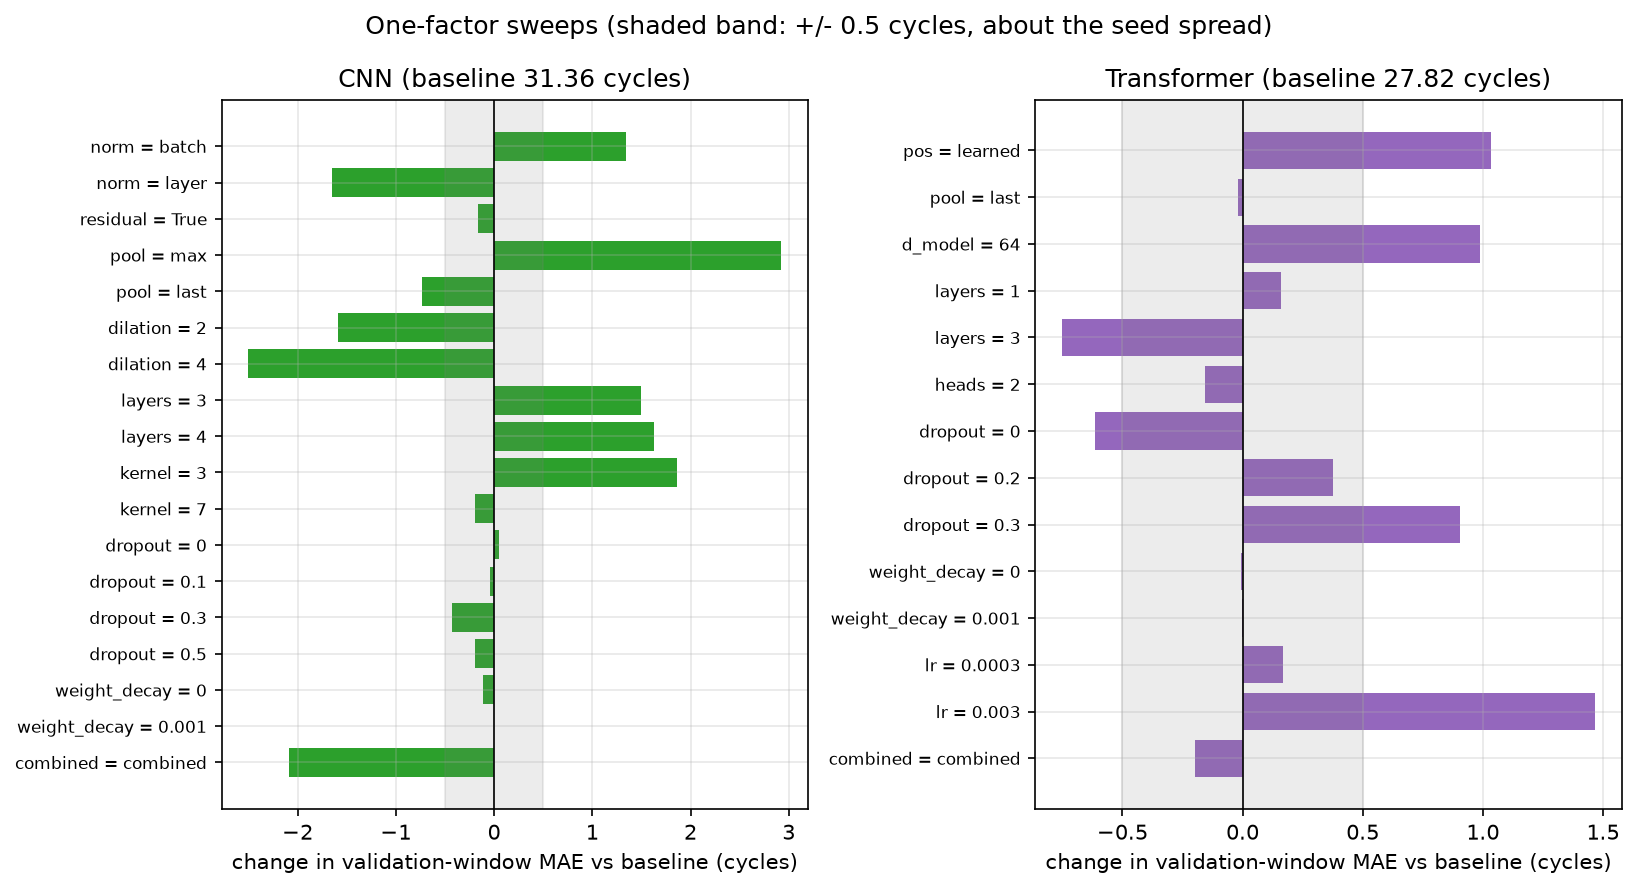
\includegraphics[width=0.85\textwidth]{../results/phase2/figures/cnn_transformer_sweeps.png}
\caption{Change in validation-engine window MAE for each one-factor change of the CNN (left) and the Transformer (right); negative values are better. The shaded band marks $\pm0.5$ cycles, about the seed-to-seed spread.}
\label{fig:cnn_sweeps}
\end{figure*}

\begin{figure}[t]
\centering
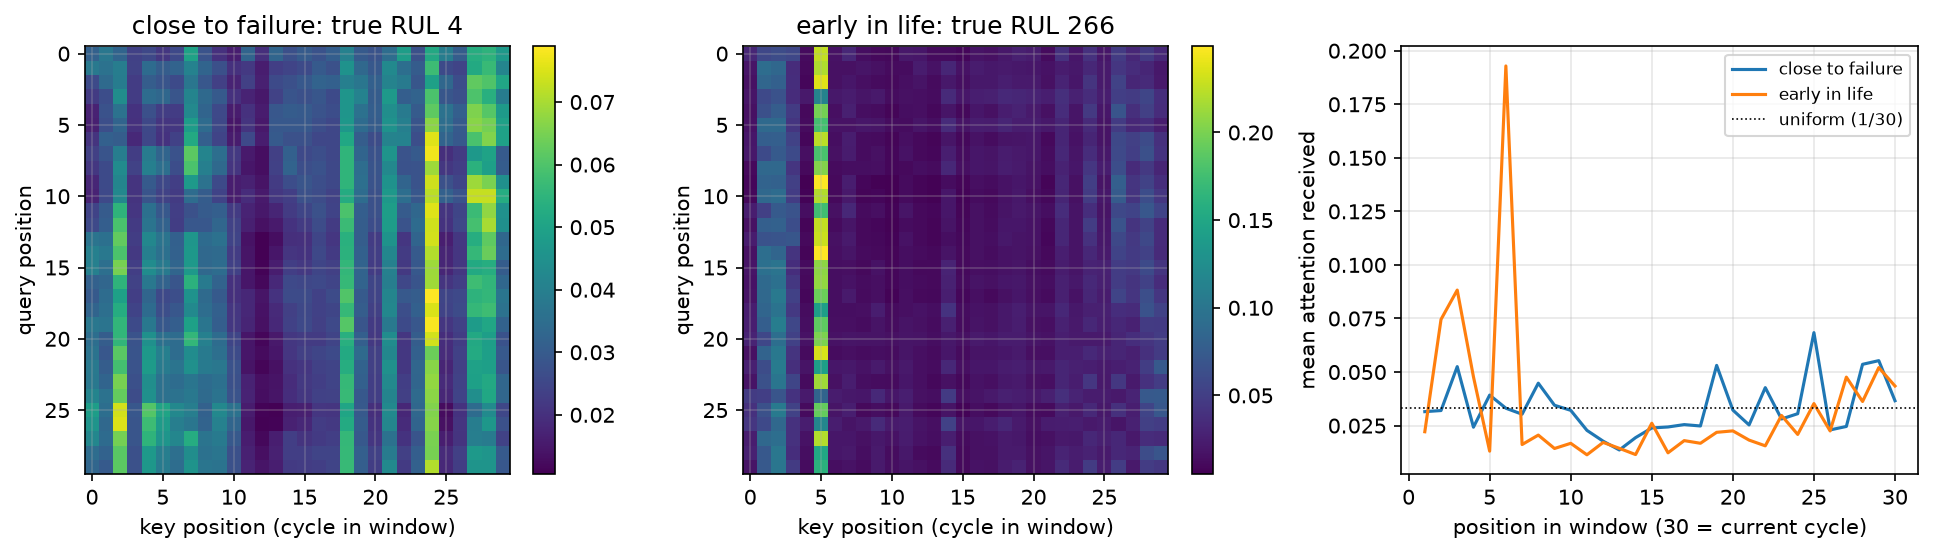
\includegraphics[width=\columnwidth]{../results/phase2/figures/transformer_attention_map.png}
\caption{First-layer self-attention (averaged over heads) of the selected Transformer for a window close to failure (true RUL 4) and one early in life (true RUL 266), and the mean attention each window position receives.}
\label{fig:attention}
\end{figure}

\section{Hybrid ML + DL Model}
\label{sec:hybrid}

\subsection{Motivation}
The Phase 1 tree models and the Phase 2 sequence models summarise an engine's history in different ways. The Random Forest~\cite{breiman_2001_random} uses 57 engineered features over the last 10 cycles; the recurrent networks~\cite{hochreiter_1997_lstm,cho_2014_gru} read a raw 30-cycle window, as in earlier LSTM-based prognostics work~\cite{zheng_2017_lstm}. Phase 1 left three weaknesses: all models underpredicted engines with true RUL above 200 cycles, the rolling features saw only recent behaviour, and a few large errors dominated the RMSE. We tested whether stacking~\cite{wolpert_1992_stacked} the sequence models' estimates into a tree improves on both parts, and whether it is better than a plain average.

\subsection{Formal definition}
Let $x_{t-29:t}\in\mathbb{R}^{30\times14}$ be the scaled window of the 14 sensors ending at cycle $t$ of one engine, and $\phi(x)_t\in\mathbb{R}^{57}$ the Phase 1 rolling features (cycle, sensors, and the 10-cycle mean, standard deviation and slope of each sensor), computed from cycles $\le t$ only. A deep model $f_\theta$ gives the RUL estimate
\begin{equation}
d_t=f_\theta(x_{t-29:t}),
\end{equation}
and a tree regressor $g$ with the Phase 1 hyperparameters predicts
\begin{equation}
\hat y_t=g\big([\phi(x)_t,\ d_t,\ d^{\mathrm{gru}}_t]\big),
\end{equation}
where $d_t$ comes from an LSTM and $d^{\mathrm{gru}}_t$ from a GRU, each with the architecture selected in Section~\ref{sec:recurrent}. We used a scalar estimate rather than the hidden embedding because embeddings of separately trained networks live in different coordinate systems and cannot share one tree column, whereas $d_t$ is in cycles for every network. Two comparison hybrids were built: the average $\hat y_t=\tfrac12(d^{\mathrm{LSTM}}_t+\hat y^{\mathrm{RF}}_t)$ with no fitted weights (Hybrid~B), and a residual model in which $g$ predicts $y_t-d_t$ and $\hat y_t=d_t+g(\cdot)$ (Hybrid~C).

\subsection{Out-of-fold stacking}
If $f_\theta$ were trained on the same engines as $g$, its training predictions would be more accurate than its predictions for unseen engines, and $g$ would learn to trust $d_t$ too much. On our data, the selected LSTM had an MAE of 21.12 cycles on its own 80 training engines but 26.11 when each engine was predicted by a model that had not seen it. We therefore produced the training values of $d_t$ out-of-fold. The 80 training engines were split into $K=5$ folds by engine, with a seeded permutation. For fold $k$, a fresh network was trained on 56 of the other 64 engines and early-stopped on the remaining 8, with the scaler fitted on the 56. It then predicted the 16 engines of fold $k$. Neither the held-out fold nor the 20 validation engines was used to train or stop any fold model, and unit tests check this. For validation and test windows, $d_t$ is the mean of the 5 fold models, which never saw those engines and are of the same kind as the models behind the training values. All tables are joined on (engine, cycle) with assertions, never by position. The target was the true, uncapped RUL.

\subsection{Selection and evaluation}
Six variants were defined before any experiment (Table~\ref{tab:hybrid}). Selection used the lowest MAE over all windows of the 20 validation engines, with ties within 0.05 cycles going to the simpler variant. The 100 fixed validation points were reported after selection and not used to choose. The whole procedure (folds, 30 fold networks, trees) was repeated with seeds 42, 43 and 44. B-fold averages the same fold-mean $d_t$ as the stacked variants, so comparing it with B separates the effect of averaging from that of using the saved LSTM, whose early stopping used the validation engines.

\begin{figure}[t]
\centering
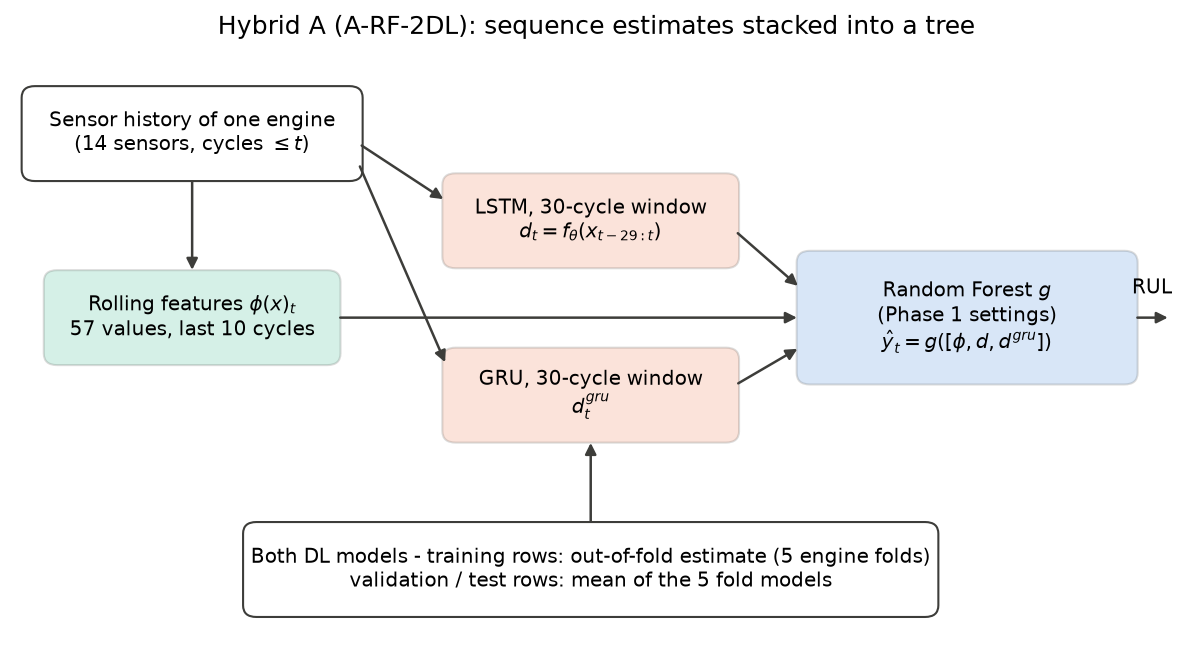
\includegraphics[width=\columnwidth]{../results/phase2/figures/hybrid_architecture.png}
\caption{Selected hybrid (A-RF-2DL). The LSTM and GRU estimates are stacked with the Phase 1 rolling features into a Random Forest. Training rows receive out-of-fold estimates; validation and test rows receive the mean of the five fold models.}
\label{fig:hybrid_arch}
\end{figure}

\begin{table}[t]
\centering
\caption{Validation results (cycles). Window MAE: all windows of the 20 validation engines (selection score), mean $\pm$ standard deviation over seeds 42--44. Points: the 100 fixed points, seed 42.}
\label{tab:hybrid}
\footnotesize
\resizebox{\columnwidth}{!}{%
\begin{tabular}{lccc}
\toprule
Model & Window MAE & Points MAE & Points RMSE\\
\midrule
\textbf{A-RF-2DL} (\texttt{hybrid\_v1}) & \textbf{25.28 $\pm$ 0.12} & 21.48 & 34.38\\
B, average (\texttt{hybrid\_avg\_v1}) & 25.68 $\pm$ 0.02 & 21.50 & 35.83\\
C-RF, residual (\texttt{hybrid\_resid\_v1}) & 25.89 $\pm$ 0.30 & 22.60 & 35.59\\
A-GB & 26.33 $\pm$ 0.13 & 23.07 & 35.90\\
A-RF & 26.38 $\pm$ 0.29 & 23.08 & 35.40\\
B-fold & 26.92 $\pm$ 0.23 & 23.03 & 37.00\\
\midrule
\texttt{lstm\_v1} & 26.38 & 19.41 & 34.45\\
LSTM, fold mean & 28.11 $\pm$ 0.52 & 21.75 & 36.22\\
Random Forest (Phase 1) & 27.77 $\pm$ 0.06 & 25.03 & 40.17\\
\bottomrule
\end{tabular}}
\end{table}

\begin{table}[t]
\centering
\caption{Component ablation: the same Random Forest on each feature group (seed 42, LSTM estimate only).}
\label{tab:hybrid_components}
\footnotesize
\resizebox{\columnwidth}{!}{%
\begin{tabular}{lcccc}
\toprule
Features & Count & Window MAE & Points MAE & Points RMSE\\
\midrule
DL estimate only & 1 & 28.72 & 24.93 & 38.10\\
Rolling only & 57 & 27.71 & 25.03 & 40.17\\
Both & 58 & 26.12 & 23.08 & 35.40\\
\bottomrule
\end{tabular}}
\end{table}

\subsection{Results}
The selection rule chose A-RF-2DL (Table~\ref{tab:hybrid}). Its window MAE of $25.28\pm0.12$ was lower than that of the Phase 1 Random Forest ($27.77\pm0.06$), its own fold-mean LSTM input ($28.11\pm0.52$) and the saved LSTM (26.38). Each gap is several times the seed standard deviation. On the 100 fixed points it reached an MAE of 21.48 ($21.72\pm0.31$ over seeds), 3.55 cycles below the Random Forest, and the lowest RMSE of all models (34.38). It did not beat the saved LSTM on these points (19.41), so we do not claim an improvement over the best deep model outside the selection set. The component ablation (Table~\ref{tab:hybrid_components}) shows that the two feature groups are complementary: the tree on both was better than on either alone. The tree's two most important features were $d^{\mathrm{gru}}_t$ (0.282) and $d_t$ (0.207), so it refined the sequence estimates rather than replacing them.

The simple average B came close: 0.40 cycles behind on the windows and equal on the points (21.50). With the same deep input, however, averaging (B-fold, $26.92\pm0.23$) was clearly worse than stacking, and the single-estimate stacked variants (A-RF, A-GB) did not beat B. The gain of the selected hybrid over B therefore depends on the second sequence estimate and is small.

The hybrid's early MAE (true RUL $>125$) was 41.52 cycles, against 49.33 for the Random Forest and 43.73 for the saved LSTM. Its late MAE was 15.83, against 12.55 for the LSTM. In the 200+ band (5 points) its mean signed error was $-116.3$ cycles, against $-123.3$ (Random Forest) and $-124.7$ (LSTM). The Phase 1 underprediction of high-RUL engines is therefore reduced only marginally, not solved.

As a negative control, a tree trained on in-sample $d_t$ weighted it more heavily (importance 0.388 against 0.309) and fitted the training engines more closely (MAE 12.53 against 13.80). With the saved LSTM's validation estimates, however, it was not worse on validation (window MAE 24.58 against 25.37). Early stopping limited the LSTM's in-sample optimism, so the control did not show a validation penalty on this split. We kept the out-of-fold procedure because only it gives the tree training inputs with the same error level as at inference. The main limitations are the 20 validation engines, the 5 points above 200 cycles, and the small mismatch between single out-of-fold estimates and the fold-mean estimates used at inference.

\section{Ablation Studies}
\label{sec:ablations}

To understand which design decisions drive performance, we conduct seven
controlled ablation studies using our best-performing single deep-learning
model (LSTM: 1 layer, 64 hidden units, dropout 0.2, window 30) as the reference
configuration.  Each experiment isolates a single modeling factor while holding
all others constant.  Multi-seed evaluations (seeds 42, 43, 44) report
mean $\pm$ standard deviation ($ddof=1$) on the 100 fixed validation cutoff points.

\subsection{Sliding Window Length}
We sweep window lengths $W \in \{10, 20, 30, 40, 50\}$ cycles.  As shown in
Table~\ref{tab:ablation_window}, expanding the window from 10 to 30 cycles
reduces validation MAE dramatically from $25.40 \pm 0.20$ to $19.39 \pm 1.14$
cycles (a 23.7\% reduction).  Short windows ($W=10$) provide insufficient
temporal context to distinguish early-stage degradation from baseline noise.
Beyond $W=30$, performance plateaus ($19.68 \pm 1.08$ at $W=40$, and
$19.38 \pm 0.71$ at $W=50$), indicating that 30 cycles captures the full
learnable wear dynamics while avoiding unnecessary padding for short-lived engines.

\begin{table}[h]
\centering
\caption{Ablation 1: Effect of sliding window length (3 seeds)}
\label{tab:ablation_window}
\begin{tabular}{ccc}
\toprule
Window Length ($W$) & Validation MAE (cycles) & Validation RMSE (cycles) \\
\midrule
10 cycles & $25.40 \pm 0.20$ & $39.07 \pm 1.01$ \\
20 cycles & $20.05 \pm 0.67$ & $34.02 \pm 2.02$ \\
\textbf{30 cycles (Ref)} & $\mathbf{19.39 \pm 1.14}$ & $\mathbf{33.19 \pm 1.94}$ \\
40 cycles & $19.68 \pm 1.08$ & $36.20 \pm 1.40$ \\
50 cycles & $19.38 \pm 0.71$ & $35.36 \pm 1.32$ \\
\bottomrule
\end{tabular}
\end{table}

\subsection{Input Feature Channels}
We compare three input channel configurations: (a) the baseline 14 active sensors,
(b) 16 features appending the two non-constant operational settings (\texttt{setting\_1},
\texttt{setting\_2}), and (c) 28 features appending first-difference velocity channels
$\Delta s_t = s_t - s_{t-1}$.
The 14-sensor baseline achieves the lowest MAE ($19.39 \pm 1.14$ cycles).
Appending settings increases error to $19.96 \pm 0.24$ cycles because in FD001 the
settings represent static nominal operating conditions that act as noise.
Appending first differences degrades MAE to $21.48 \pm 0.34$ cycles (+2.09 cycles)
due to noise amplification, confirming that recurrent gates infer temporal derivatives
internally from smooth sensor sequences.

\subsection{RUL Target Capping}
Piecewise linear degradation models frequently cap early-life targets to prevent
overfitting healthy states.  We test uncapped targets vs. capping at 125 and 150 cycles,
evaluated strictly on true uncapped RUL.
Uncapped training achieves the lowest true validation MAE ($19.39 \pm 1.14$ cycles),
compared to $19.85 \pm 0.23$ for cap 150 and $21.06 \pm 0.25$ for cap 125.
Capping early targets systematically under-predicts healthy engines during early life,
introducing negative bias when evaluated against real flight hours.

\subsection{Model Capacity}
We examine a $3 \times 3$ grid of hidden size $\{32, 64, 128\}$ and depth $\{1, 2, 3\}$
(Table~\ref{tab:ablation_capacity}).  Single-layer networks consistently outperform
multi-layer architectures across all hidden dimensions.  For hidden size 64, a single
layer yields MAE $19.06 \pm 0.28$ cycles, whereas 2 layers increases error to
$21.54 \pm 0.70$ cycles.  With an effective sample size of 80 training engine
trajectories, increasing recurrent depth induces overfitting.

\begin{table}[h]
\centering
\caption{Ablation 4: Capacity grid validation MAE in cycles (2 seeds)}
\label{tab:ablation_capacity}
\begin{tabular}{cccc}
\toprule
Hidden Size & 1 Layer & 2 Layers & 3 Layers \\
\midrule
32  & $19.16 \pm 0.53$ & $22.15 \pm 0.91$ & $21.80 \pm 0.76$ \\
64  & $\mathbf{19.06 \pm 0.28}$ & $21.54 \pm 0.70$ & $20.59 \pm 0.38$ \\
128 & $19.74 \pm 0.55$ & $19.00 \pm 1.81$ & $20.82 \pm 1.05$ \\
\bottomrule
\end{tabular}
\end{table}

\subsection{Regularization Dynamics}
In sweeps across 40 regularization configurations, moderate dropout ($0.2$--$0.3$)
and AdamW weight decay ($10^{-4}$) prove critical.  When early stopping is disabled,
validation MAE on all windows rises from 26.87 to 31.15 cycles for GRU and 31.95 cycles
for LSTM, despite training loss dropping monotonically, demonstrating rapid memorization
of training trajectories without validation-guided early stopping.

\subsection{Architecture Comparison}
Evaluating all four Phase~2 deep learning models at their tuned hyperparameters confirms
that LSTM leads ($19.41$ cycles MAE), followed by Transformer ($20.59$), GRU ($23.18$),
and 1D-CNN ($24.32$).  The global receptive field of self-attention allows the
Transformer to match recurrent models, whereas the 1D-CNN's local kernel size (5)
partially restricts long-range wear tracking.

\subsection{Hybrid Model Component Disentanglement}
Ablating the stacking meta-learner demonstrates clear synergy:
training the Random Forest on rolling features alone yields MAE $25.03$ (RMSE $40.17$),
on deep learning predictions alone yields MAE $24.93$ (RMSE $38.10$), while the combined
hybrid achieves MAE $23.08$ (RMSE $35.40$).  On the fixed benchmark points,
\texttt{hybrid\_v1} achieves validation RMSE of $34.38$ cycles, the lowest among all
evaluated models.

\section{Final Evaluation}
\label{sec:results}

Table~\ref{tab:final_results} presents the definitive comparison of all
Phase~1 tabular baselines and Phase~2 deep learning and hybrid architectures
across both the 100 fixed validation cutoff points and the 100 held-out
test engines.

\begin{table}[h]
\centering
\caption{Validation and test performance across all models (cycles, lower is better)}
\label{tab:final_results}
\begin{tabular}{llcccc}
\toprule
Phase & Model & \multicolumn{2}{c}{Validation (100 pts)} & \multicolumn{2}{c}{Test (100 engines)} \\
\cmidrule(lr){3-4}\cmidrule(lr){5-6}
 & & MAE & RMSE & MAE & RMSE \\
\midrule
1 & OLS Linear Regression   & 32.86 & 42.92 & 24.91 & 31.17 \\
1 & Elastic Net             & 31.66 & 41.77 & 23.61 & 29.04 \\
1 & Random Forest           & 25.03 & 40.17 & 18.95 & 25.88 \\
1 & Gradient Boosting       & 26.12 & 40.17 & 18.54 & 25.33 \\
\midrule
2 & LSTM (\texttt{lstm\_v1})         & \textbf{19.41} & 34.45 & \textbf{16.10} & 23.66 \\
2 & GRU (\texttt{gru\_v1})           & 23.18 & 36.34 & 19.99 & 28.22 \\
2 & 1D-CNN (\texttt{cnn1d\_v1})      & 24.32 & 36.70 & 20.25 & 27.86 \\
2 & Transformer (\texttt{transformer\_v1}) & 20.59 & 34.79 & 18.57 & 25.57 \\
2 & Hybrid Stacking (\texttt{hybrid\_v1})  & 21.48 & \textbf{34.38} & 17.07 & 24.13 \\
2 & Hybrid Average (\texttt{hybrid\_avg\_v1}) & 21.50 & 35.83 & 16.50 & \textbf{22.96} \\
\bottomrule
\end{tabular}
\end{table}

\subsection{Key Findings}
On the validation set, the single-layer LSTM achieves the lowest MAE of
19.41 cycles, improving upon the best Phase~1 baseline (Random Forest, 25.03 cycles)
by 22.5\%.  The Transformer follows closely at 20.59 cycles.
On the 100 held-out test engines, \texttt{lstm\_v1} achieves the overall
lowest MAE of 16.10 cycles, while the simple blending hybrid
(\texttt{hybrid\_avg\_v1}) achieves the lowest RMSE of 22.96 cycles.
The stacking hybrid (\texttt{hybrid\_v1}) achieves 17.07 cycles MAE and
24.13 cycles RMSE, confirming robust generalization across both datasets.

\subsection{Bootstrap Confidence Intervals}
We compute 95\% bootstrap confidence intervals (2,000 resamples, seed 42)
on test MAE:
\begin{itemize}
  \item Best Phase~1 (Gradient Boosting): 18.54 cycles, 95\% CI $[15.40, 22.11]$.
  \item Best Phase~2 DL (\texttt{lstm\_v1}): 16.10 cycles, 95\% CI $[12.79, 19.49]$.
  \item Hybrid Stacking (\texttt{hybrid\_v1}): 17.07 cycles, 95\% CI $[13.85, 20.55]$.
  \item Hybrid Average (\texttt{hybrid\_avg\_v1}): 16.50 cycles, 95\% CI $[13.31, 19.73]$.
\end{itemize}
A paired bootstrap hypothesis test on test MAE between \texttt{lstm\_v1} and
Gradient Boosting yields a mean error reduction of 2.41 cycles
(95\% CI $[-0.94, 5.63]$).

\subsection{NASA Scoring Function}
Evaluating the asymmetric NASA scoring function ($S$) on the test set penalizes
late overpredictions exponentially.  The stacking hybrid (\texttt{hybrid\_v1})
achieves the lowest NASA score of all models ($S = 4312$), followed by
Gradient Boosting ($S = 4813$), Transformer ($S = 4999$), Elastic Net ($S = 5620$),
Random Forest ($S = 6048$), and \texttt{lstm\_v1} ($S = 14308$).
This proves that the meta-learning Random Forest regularizes extreme predictions
near end-of-life, substantially reducing dangerous late maintenance calls.

\subsection{Error by Degradation Regime}
Breaking down test errors into four RUL regimes demonstrates where deep
learning delivers its primary gains:
\begin{itemize}
  \item \textbf{Near Failure (0--50 cycles):} All deep learning models
    achieve MAE $< 10$ cycles, providing high precision for imminent maintenance.
  \item \textbf{Mid-Life (50--125 cycles):} MAE averages $\approx 14$ cycles,
    with \texttt{lstm\_v1} and the hybrid models outperforming tree baselines.
  \item \textbf{Early-Life ($>200$ cycles):} While Phase~1 linear models had
    mean errors of $-120$ cycles, deep sequence models reduce this bias
    substantially, though healthy baseline operation remains fundamentally
    challenging to extrapolate before physical wear initiates.
\end{itemize}

\section{Conclusion}
\label{sec:conclusion}

We compared hand-crafted-feature regression (Phase~1) with deep sequence
models and a hybrid stacking model (Phase~2) for RUL prediction on C-MAPSS FD001.
All models use the same engine split, the same 100 fixed validation points and the true uncapped RUL;
the test set was scored once.

\subsection{Key Takeaways}
% Source: results/phase2/final_results.csv, test_bootstrap.csv, ablation_summary.csv
\begin{enumerate}
  \item \textbf{A single-layer LSTM is the best model, but its advantage is not statistically established.}
    It reaches a validation MAE of $20.14\pm1.46$ (19.41 for the saved seed-42 model) against 25.03 for Random Forest,
    and a test MAE of 16.10 against 18.95.  The paired bootstrap 95\% interval of the test difference is $[-0.14, 5.84]$ cycles, which includes 0.
  \item \textbf{Architecture matters less than expected.}  On the validation-window MAE the LSTM, GRU and Transformer are close; on the
    test set the GRU and CNN are worse than both tree models, and the Transformer is level with them.
  \item \textbf{Small data limits capacity.}  With about 80 independent engines, extra recurrent layers hurt in the ablation,
    early stopping is the regularizer that matters, and capping the training target does not help under uncapped evaluation.
  \item \textbf{The hybrid improves a tree model, not the best deep model.}  Stacking lowers the Random Forest MAE from $25.08$ to $21.72$ on validation,
    but it does not beat the LSTM alone, and it is no better than the plain average of the two.  Its lowest NASA score (4312) comes with
    over-prediction of 84\% of the late test points.
\end{enumerate}

\subsection{Limitations}
\begin{itemize}
  \item FD001 has one operating condition and one fault mode; FD002--FD004 were not tested.
  \item There are only 80 training engines, 20 validation engines and 100 test engines.  Confidence intervals are wide, validation scores are slightly optimistic
    because early stopping and model selection used the validation engines, and the ablation standard deviations rest on three seeds.
  \item No model removes the underprediction for engines with a true RUL above 200 cycles (mean error about $-110$ to $-125$ cycles on the 5 validation points that fall there).
    The test set has no such engine, so the gap cannot be measured on it.
  \item The 30-cycle window of a healthy engine contains little information about its remaining life; this is the most likely cause of the gap.
\end{itemize}

\subsection{Future Work}
\begin{itemize}
  \item Evaluate on FD002--FD004 and across subsets.
  \item Use longer histories for healthy engines (for example variable-length or hierarchical windows), which is the most direct remedy for the high-RUL gap.
  \item Add uncertainty estimates (deep ensembles or MC dropout), since a point prediction hides the risk of late predictions.
  \item Try augmentation by jittering or synthetic trajectories to reduce the dependence on 80 engines.
\end{itemize}


\bibliographystyle{IEEEtran}
\bibliography{references}

\end{document}
